% LaTex styling for this file was generated by ChatGPT4.0. The instructions were written by the authors and was NOT generated.

\documentclass[12pt,a4paper]{article}

% Packages
\usepackage[margin=1in]{geometry}
\usepackage{graphicx}
\usepackage{float}
\usepackage{hyperref}
\usepackage{booktabs}
\usepackage{tabularx}
\usepackage{array}
\usepackage{caption}
\usepackage{xurl}
\usepackage{enumitem}

% Code block formatting
\usepackage{listings}
\usepackage{xcolor}

% Define code colours
\definecolor{codebackground}{RGB}{245,246,248}
\definecolor{codeblue}{RGB}{35,90,160}
\definecolor{codegreen}{RGB}{40,125,80}
\definecolor{codegray}{RGB}{100,100,100}
\definecolor{codepurple}{RGB}{130,70,150}

% Configure code listings
\lstdefinestyle{terminal}{
    backgroundcolor=\color{codebackground},
    basicstyle=\ttfamily\small,
    keywordstyle=\color{codeblue}\bfseries,
    commentstyle=\color{codegreen}\itshape,
    stringstyle=\color{codepurple},
    numbers=none,
    breaklines=true,
    breakatwhitespace=false,
    showstringspaces=false,
    frame=single,
    rulecolor=\color{codegray!30},
    frameround=tttt,
    tabsize=4,
    keepspaces=true,
    columns=fullflexible,
    xleftmargin=5pt,
    xrightmargin=5pt,
    aboveskip=10pt,
    belowskip=10pt
}

\lstdefinestyle{terminaloutput}{
    backgroundcolor=\color{codebackground},
    basicstyle=\ttfamily\small\color{codegray},
    numbers=none,
    breaklines=true,
    frame=single,
    rulecolor=\color{codegray!30},
    frameround=tttt,
    keepspaces=true,
    columns=fullflexible,
    xleftmargin=5pt,
    xrightmargin=5pt,
    aboveskip=10pt,
    belowskip=10pt
}


% Hyperlink formatting
\hypersetup{
    colorlinks=true,
    linkcolor=blue,
    urlcolor=blue,
    citecolor=blue
}

% Document information
\title{Build Guide for Tree Imaging Machine}
\author{}
\date{}

\begin{document}

\maketitle

% Automatically generated table of contents
\tableofcontents
\newpage

% --------------------------------------------------
\section{Installing Jetson Linux 36.3.0 and Other Software Dependencies}

\subsection{Download Drivers and Follow NVIDIA Quick Start Guide}
Jetson Linux 36.3.0 must first be installed on the Jetson Orin Nano Developer Kit using an x86-based computer running Ubuntu 22.04 or Ubuntu 20.04.

\begin{enumerate}
    \item Download the \textit{Driver Package (BSP)} and \textit{Sample Root Filesystem} for \href{https://developer.nvidia.com/embedded/jetson-linux-r363}{Jetson Linux 36.3.0} onto an x86 Ubuntu 22.04 or Ubuntu 20.04 computer.

    \item Follow the \href{https://docs.nvidia.com/jetson/archives/r36.3/DeveloperGuide/IN/QuickStart.html}{NVIDIA Quick Start Guide}. Ensure that the environment variables for the Driver Package and Root Filesystem point to the correct file paths on your computer.
    \item Connect the Jetson to a computer monitor, keyboard, and mouse.
    \item Complete the first-boot setup. Once the Jetson has booted, confirm the installed Jetson Linux version by running the following command in the terminal:
\end{enumerate}

\begin{lstlisting}[style=terminal]
cat /etc/nv_tegra_release
\end{lstlisting}

The terminal should display output similar to the following, indicating that Jetson Linux Version 36.3 has been installed:

\begin{lstlisting}[style=terminaloutput]
# R36 (release), REVISION:3.0, ...
\end{lstlisting}

\subsection{Connect the Raspberry Pi HQ Camera to the Jetson}

The Raspberry Pi HQ Camera is now ready to be connected to the Jetson. 

\begin{enumerate}
    \item Unplug the Jetson from any power source.
    \item Take out the 15 to 22 pin flexible camera cable. 
    \item Pull on the plastic pull tab on the CAM1 connector of the Jetson to open the connector.
    \item Insert the narrower, 22 pin end of the cable into the connector, making sure the metal contacts are facing the circuit board, NOT the sky. Push in the plastic tab to secure the cable. 
    \item Pull on the plastic pull tab on the connector on the Raspberry Pi HQ Camera to open the connector.
    \item Insert the wider, 15 pin end of the cable into the camera connector, making sure the metal contacts are facing the circuit board, NOT the sky. Push in the plastic tab to secure the cable. 
\end{enumerate}

% ==================================================
\subsection{Downloading the GitHub Repository}

Once Jetson Linux has been installed, the TIM GitHub repository must be downloaded onto the Jetson.

\begin{enumerate}
    \item Log into the Jetson and connect to the internet using Wi-Fi or Ethernet.

    \item Clone the TIM GitHub repository using Git:
\end{enumerate}

\begin{lstlisting}[style=terminal,language=bash]
git clone https://github.com/ANONYMIZED/REPO
cd REPO
\end{lstlisting}

% ==================================================
\subsection{Installing Dependencies Using Docker}

The TIM system is designed to be ran inside a Docker container for ease of installation and portability. If you enter any command and receive a permission error, run the same command with \texttt{sudo} at the beginning and enter your password when prompted.

\begin{enumerate}
    \item Make the build, launch, and entrypoint scripts executable:
\end{enumerate}

\begin{lstlisting}[style=terminal,language=bash]
chmod +x build.sh launch.sh entrypoint.sh
\end{lstlisting}

\begin{enumerate}[resume]
    \item Run the build script to install the required dependencies. This process may take several minutes:
\end{enumerate}

\begin{lstlisting}[style=terminal,language=bash]
./build.sh
\end{lstlisting}

\begin{enumerate}[resume]
    \item The launch script will start a new Docker container with the necessary dependencies. Once the container launches, the terminal environment will change to the Docker container.
\end{enumerate}

\begin{lstlisting}[style=terminal,language=bash]
./launch.sh
\end{lstlisting}

\begin{enumerate}[resume]
    \item Start the Python GUI by running the following command inside the Docker container. This will launch two windows: one displaying the live camera viewer and another displaying the user interface. 
\end{enumerate}

\begin{lstlisting}[style=terminal,language=bash]
python gui.py
\end{lstlisting}


% ==================================================
\subsection{Checking if the Docker Container is Running}

Another way to confirm that the Docker container is running, open a new terminal tab without closing the terminal currently running the \texttt{./launch.sh} process. Run the following command in the new terminal:

\begin{lstlisting}[style=terminal,language=bash]
sudo docker ps
\end{lstlisting}
This will display a list of currently active Docker containers. Confirm that the project container is listed.

% Add installation instructions here.

% --------------------------------------------------
\section{Assembling the ACRO Motion Kit}

\subsection{OpenBuilds ACRO 1010 Kit + OpenBuilds Linear Actuator Kit + OpenBuilds BlackBox Motor Controller}

We based our design on the OpenBuilds ecosystem, relying on their motion kits and motor controller. You must follow their instructions for the initial assembly steps. They are detailed below.

\begin{enumerate}
    \item Assemble the ACRO by following the assembly video made by OpenBuilds (\href{https://www.youtube.com/watch?v=YDLJrxrMEAo}{OpenBuilds, 2019a}).

    \item Assemble the linear actuator by following the assembly video made by OpenBuilds (\href{https://www.youtube.com/watch?v=X0Z_gfl-iGY}{OpenBuilds, 2018}). The linear actuator will eventually need to be attached to the X and Y planes, as described in later steps.

    \item Follow the electrical assembly instruction video made by OpenBuilds (\href{https://www.youtube.com/watch?v=GrjqW2MDCvM}{OpenBuilds, 2019b}).
\end{enumerate}

After following these detailed videos, you will have a complete motion system connected to the BlackBox. The controller is ready to receive G-code commands to guide its motion. Testing motion is described in Section \ref{sec:testing-motion}.

\subsection{Attach the OpenBuilds V-Slot NEMA 17 Linear Actuator to the ACRO}

The ACRO needs the linear actuator to be attached with custom adapters to include motion in the Z direction.

\subsection{Alternative Motion Kit Suggestions}

Motion kits are subject to market availability. There are many kits available, and the most suitable options are sold as CNC router kits, which can be readily adapted to hold a camera and Jetson Orin Nano. So long as the motor controller has GRBL firmware, it will be compatible with the commands that TIM uses to control the motion. Assembly instructions vary by kit. Adapters must be designed and 3D printed to fit any kit other than the OpenBuilds ACRO. Please write a GitHub Issue if you don't know where to start in order to design a 3D-printed bracket for your machine kit.

\begin{table}[htbp]
\centering
\begin{tabularx}{\textwidth}{p{3.2cm} p{2.6cm} p{1.5cm} p{1.5cm} p{1.4cm} X}
\toprule
\textbf{Product Name} & \textbf{Manufacturer} & \textbf{City} & \textbf{Country} & \textbf{Price (CAD)} & \textbf{Product Link} \\
\midrule

4040-PRO Desktop CNC Router
(400 $\times$ 400 $\times$ 78 mm)
& Genmitsu
& Lenexa
& USA
& \$752
& \href{https://www.sainsmart.com/products/genmitsu-4040-pro-semi-assembly-desktop-cnc-machine-for-carving-and-cutting?variant=40277984247887}{Genmitsu} \\

FoxAlien Masuter Pro 3-Axis CNC Router
(400 $\times$ 400 $\times$ 60 mm)
& FoxAlien
& Dongguan
& China
& \$670
& \href{https://www.amazon.ca/dp/B09ZTYGGTJ}{Amazon Canada} \\

VEVOR CNC Router 300W, 3-Axis
(400 $\times$ 400 $\times$ 75 mm)
& VEVOR
& Shanghai
& China
& \$550
& \href{https://www.amazon.ca/dp/B0CDW779Q6}{Amazon Canada} \\

\midrule
\multicolumn{6}{l}{\textbf{Optional Extension Kits}} \\

4040-PRO Working Area Extension Kits
& Genmitsu
& Lenexa
& USA
& \$200 to \$400
& \href{https://www.sainsmart.com/products/xy-extension-kit-for-4040-pro}{Genmitsu} \\

\bottomrule
\end{tabularx}
\caption{Alternative CNC motion kits and available extension options.}
\label{tab:alternative-cnc-kits}
\end{table}

% --------------------------------------------------
\section{Testing XYZ Motion with Universal G-Code Sender Platform}
\label{sec:testing-motion}

% Add motion testing instructions here.
\url{https://github.com/winder/Universal-G-Code-Sender/wiki/Usage#ugs-platform}

% --------------------------------------------------
\section{Install Adapters, Jetson, and Camera to the ACRO}

\subsection{Attaching Leg Extensions}
\label{subsec:attaching-legs}

Add additional height to the ACRO using aluminum extrusion. Use the corner brackets to connect the aluminum extrusions and form the legs as seen in FIgure \ref{fig:leg-height-tool}. The 3D-printed leg height tool makes it easy to ensure that all four legs are the same length. The necessary components are listed in Table \ref{tab:leg-components}.

\begin{figure}[H]
    \centering
    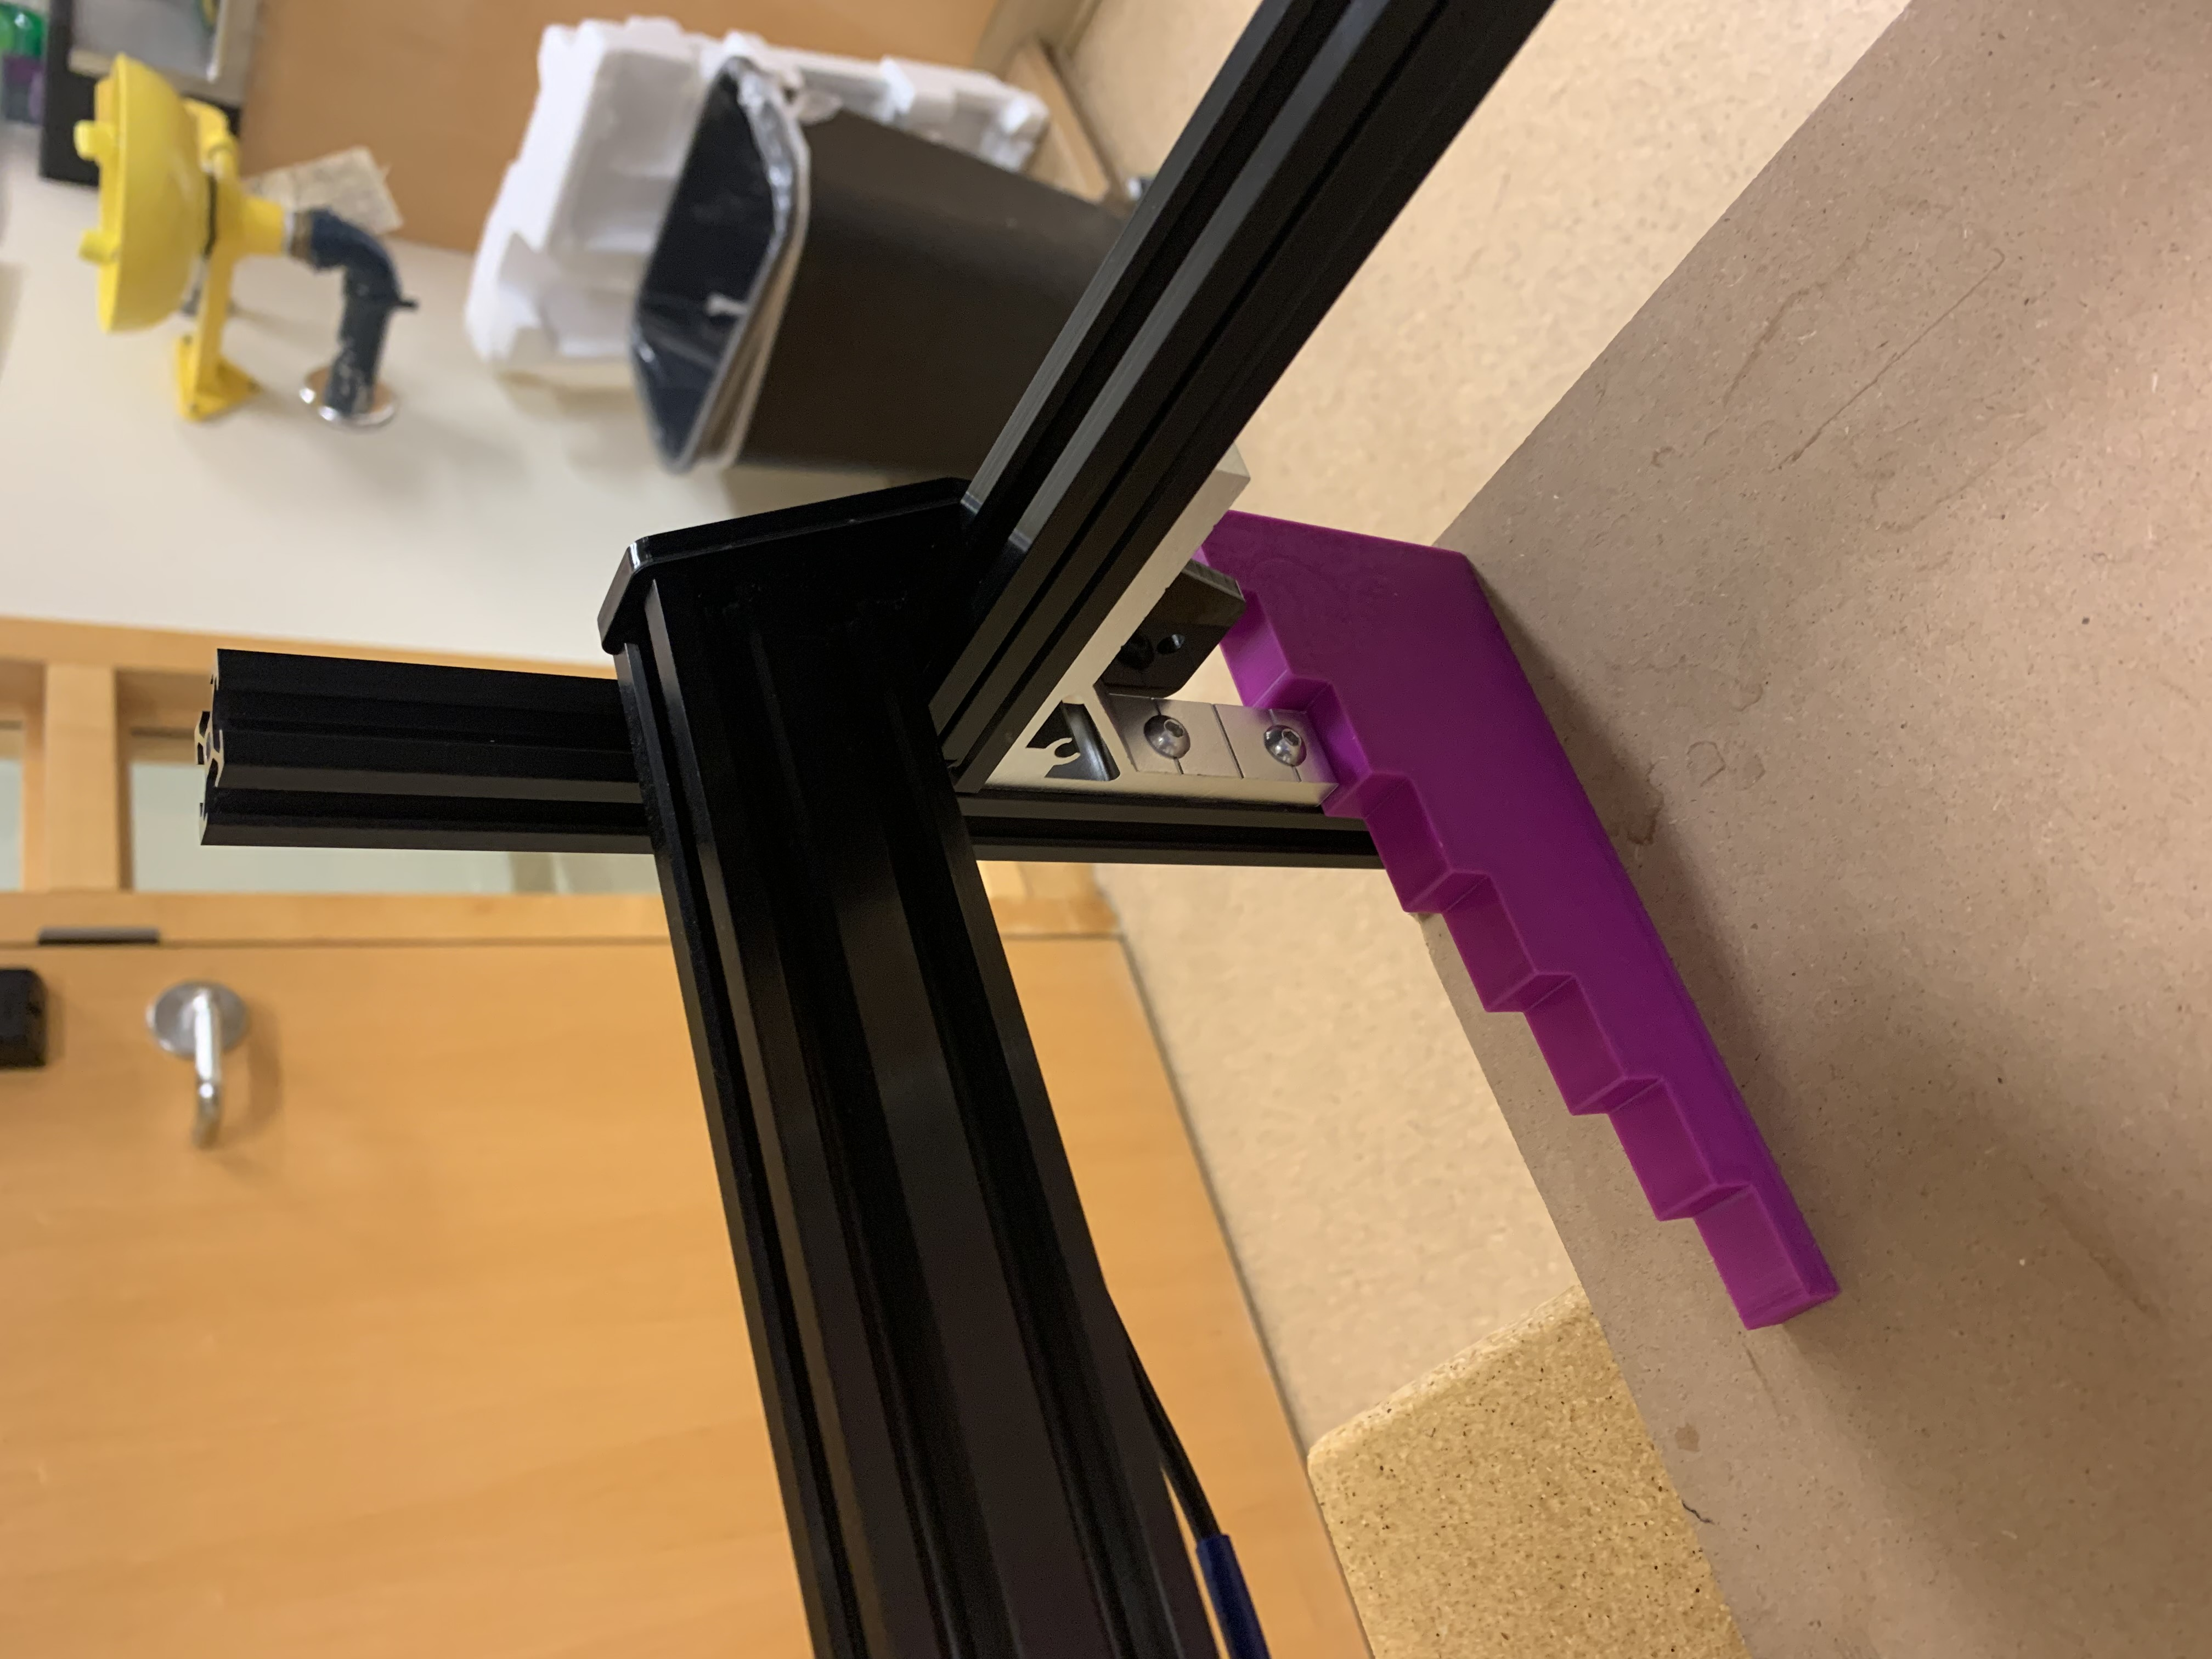
\includegraphics[width=0.5\textwidth, angle=-90]{../docs/content/leg_tool.jpg}
    \caption{3D-printed leg height tool used to ensure consistent leg lengths.}
    \label{fig:leg-height-tool}
\end{figure}

\begin{table}[H]
\centering
\begin{tabularx}{\textwidth}{p{2.5cm} X c}
\toprule
\textbf{Component Type} & \textbf{Component Name} & \textbf{Quantity} \\
\midrule

3D Prints &
\href{https://3d.nih.gov/entries/3DPX-021561}{leg\_height\_tool.stl} & 1 \\

\midrule
Hardware & M4 $\times$ 12 mm bolts & 16 \\
         & M4 hammer head t nuts & 16 \\

\midrule
Extra & Extruded aluminum corner brackets & 4 \\
      & 250 mm $\times$ 20 mm $\times$ 20 mm aluminum extrusion & 4 \\

\bottomrule
\end{tabularx}
\caption{Components required for attaching the ACRO legs.}
\label{tab:leg-components}
\end{table}


% ==================================================
\subsection{Attaching the Camera and Computer Adapter}
\label{subsec:camera-computer-adapter}

Bolt on the camera and computer adapters to the linear actuator kit using bolts and locknuts. The exploded view of the assembly is shown in Figure \ref{fig:camera-lens-holder}. The necessary components are listed in Table \ref{tab:camera-adapter-components}.

\begin{figure}[H]
    \centering
    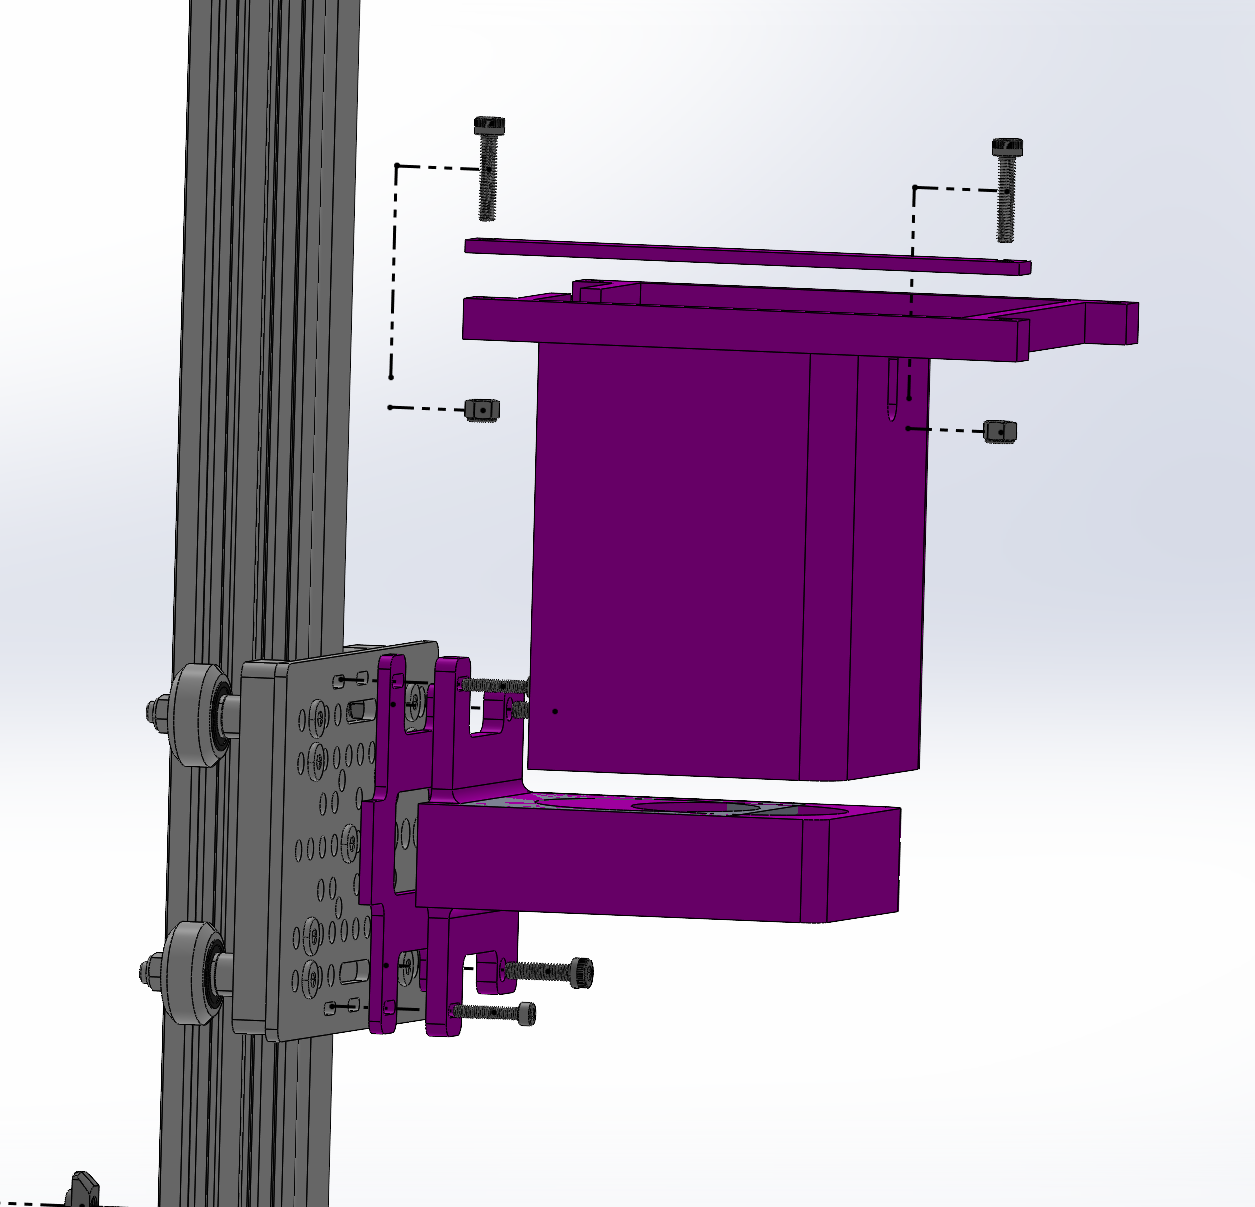
\includegraphics[width=0.5\textwidth]{../docs/content/camera_lens_holder_exploded.png}
    \caption{Exploded view of the camera and computer adapter assembly.}
    \label{fig:camera-lens-holder}
\end{figure}

\begin{table}[H]
\centering
\begin{tabularx}{\textwidth}{p{2.5cm} X c}
\toprule
\textbf{Component Type} & \textbf{Component Name} & \textbf{Quantity} \\
\midrule

3D Prints &
\href{https://3d.nih.gov/entries/3DPX-021561}{z\_axis\_plate\_adapter.stl} & 1 \\

& z\_axis\_plate\_spacer.stl & 1 \\

& z\_axis\_jetson\_carriage.stl & 1 \\

& z\_axis\_jetson\_lock.stl & 1 \\

\midrule
Hardware & M3 $\times$ 16 mm bolts & 2 \\
         & M3 locknuts & 2 \\
         & M4 $\times$ 16 mm bolts & 2 \\
         & M4 locknuts & 2 \\

\midrule
Extra & OpenBuilds Linear Actuator attachment plate & 1 \\

\bottomrule
\end{tabularx}
\caption{Components required for the camera and computer adapter.}
\label{tab:camera-adapter-components}
\end{table}

% ==================================================
\subsubsection{Attaching the Z Axis}
\label{subsubsec:attaching-z-axis}

The linear actuator needs to be connected to the ACRO gantry to allow for motion in the Z direction. Use the hammer head t-nuts to mount into the aluminum extrusion of the linear actuator. The exploded view of the assembly is shown in Figure \ref{fig:z-axis-plate}. The necessary components are listed in Table \ref{tab:z-axis-components}.

\begin{figure}[H]
    \centering
    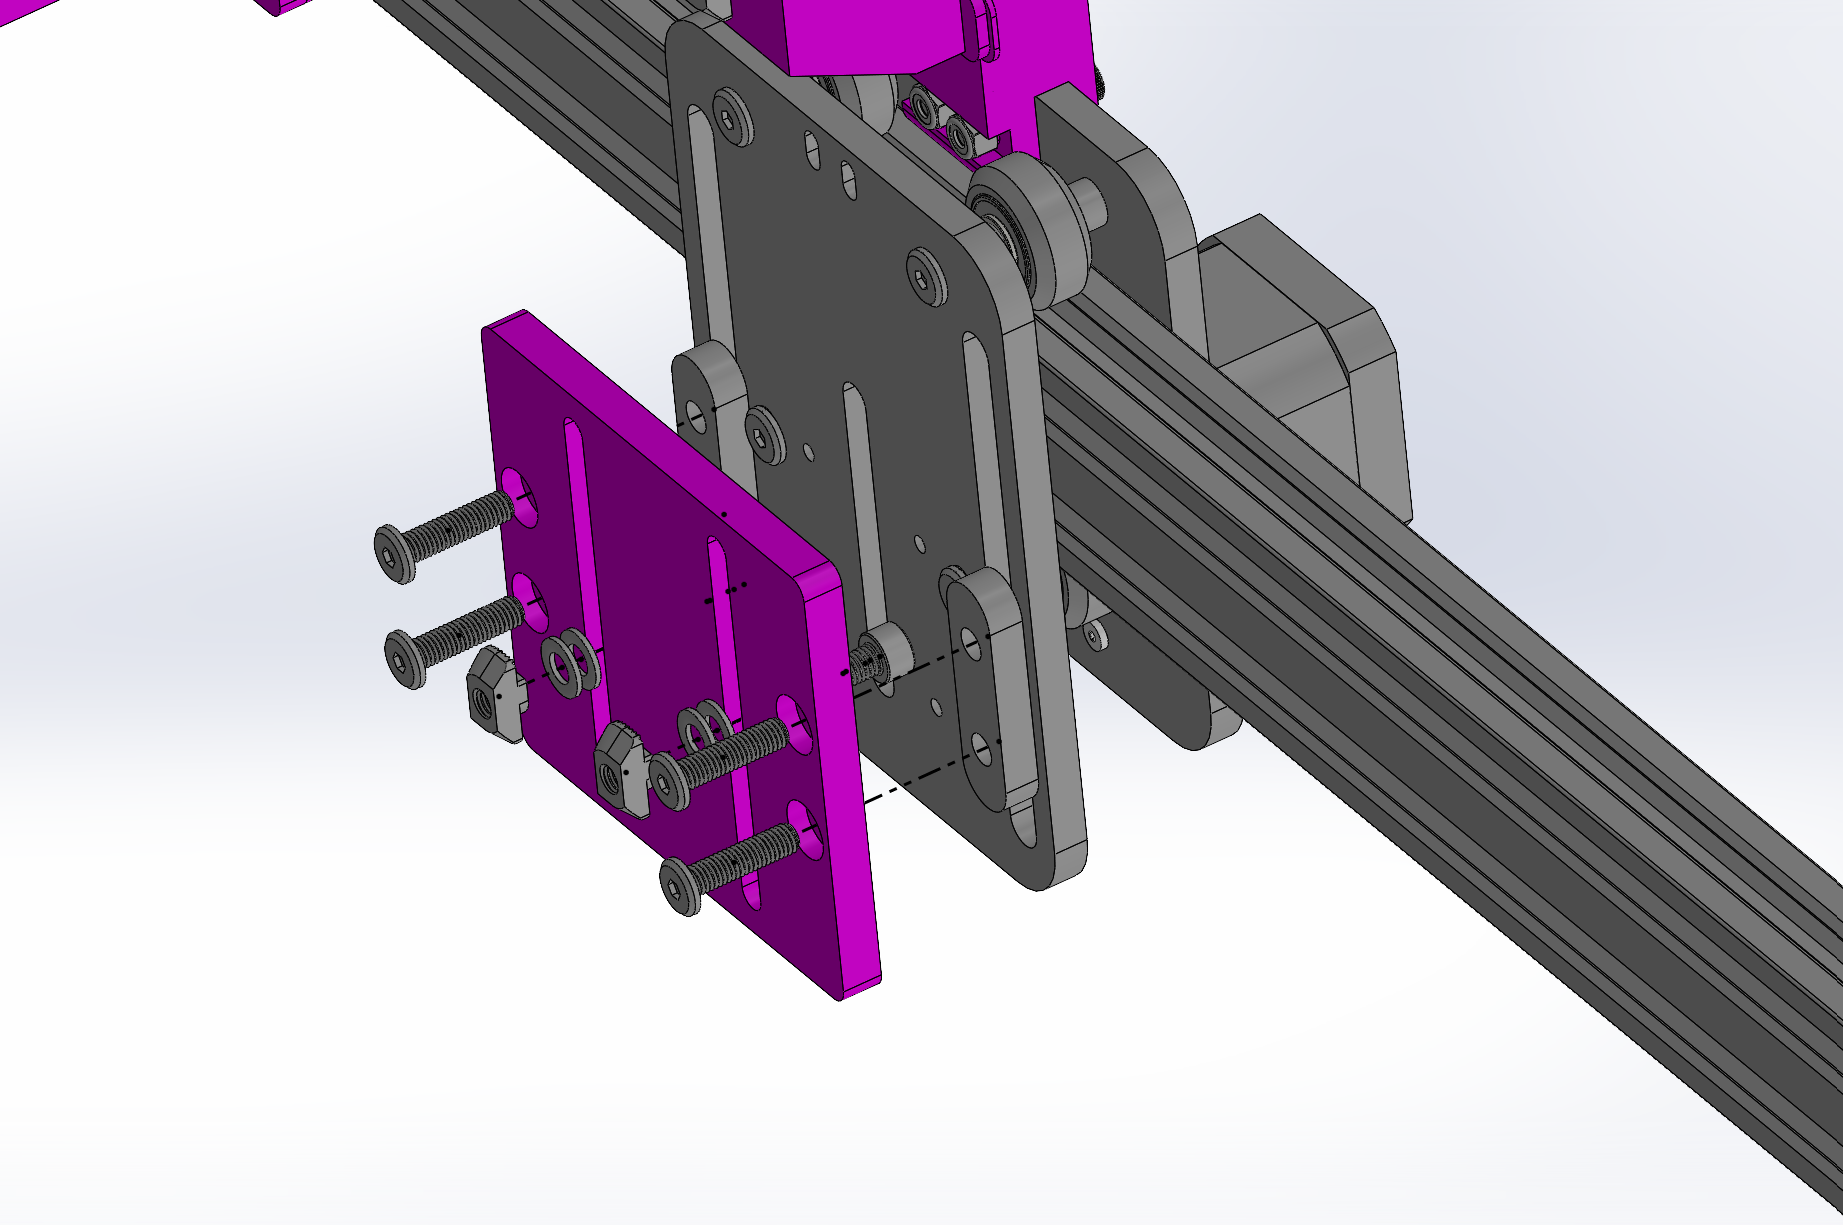
\includegraphics[width=0.5\textwidth]{../docs/content/z_axis_plate_exploded.png}
    \caption{Exploded view of the Z-axis adapter assembly.}
    \label{fig:z-axis-plate}
\end{figure}

\begin{table}[H]
\centering

\begin{tabularx}{\textwidth}{p{2.5cm} X c}
\toprule
\textbf{Component Type} & \textbf{Component Name} & \textbf{Quantity} \\
\midrule

3D Prints &
\href{https://3d.nih.gov/entries/3DPX-021561}{z\_axis\_adapter.stl} & 1 \\

& lens\_plate\_spacer.stl & 1 \\

\midrule
Hardware & M5 $\times$ 16 mm bolts & 2 \\
         & M5 T-nuts & 2 \\
         & M5 washers & 6 \\

\midrule
Extra & OpenBuilds Linear Actuator & 1 \\

\bottomrule
\end{tabularx}
\caption{Components required for attaching the Z axis.}
\label{tab:z-axis-components}
\end{table}

The attachment plate supplied with the ACRO is not designed to easily connect to the linear actuator. To address this, we designed a custom Z-axis adapter with slots that align with the aluminum extrusion.

The washers are used as spacers to shim between the bolts and the adapter, allowing adjustments to the effective bolt length and ensuring a secure fit.

% ==================================================
\subsection{Torsion Correction}
\label{subsec:torsion-correction}

The additional weight of the computer, camera, lens, and linear actuator results in some torsional deflection of the ACRO gantry. It is important for the camera to be parallel to the surface on which the samples are placed to ensure consistent image acquisition. To compensate for deflection in the gantry beam, the torsion correction system allows shims to be added or removed. These shims adjust the angle of the linear actuator relative to the imaging table. You can rotate the Z-axis by removing or adding shims as necessary. Use a bullet level to verify that the camera assembly is level relative to the imaging surface. The exploded view of the torsion correction assembly is shown in Figure \ref{fig:torsion-correction}. The necessary components are listed in Table \ref{tab:torsion-components}.

\begin{figure}[H]
    \centering
    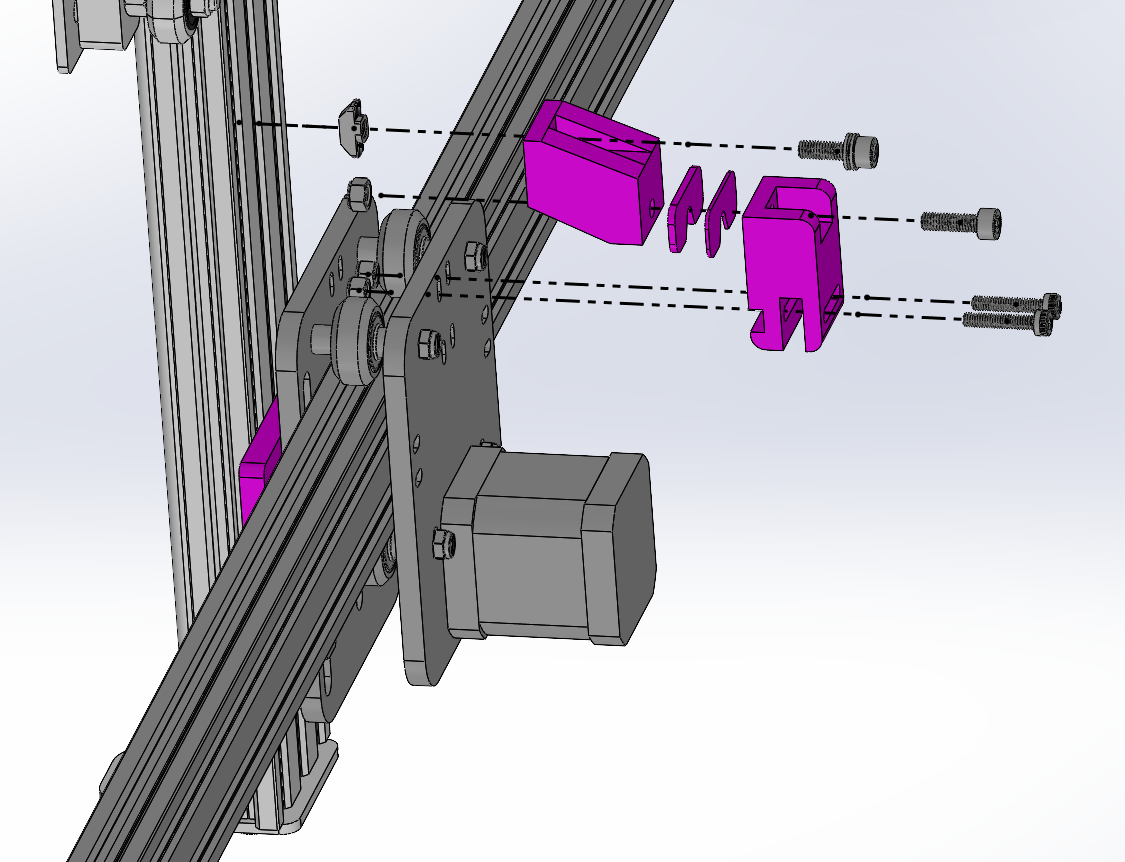
\includegraphics[width=0.5\textwidth]{../docs/content/torsion_correction_exploded.png}
    \caption{Exploded view of the torsion correction assembly.}
    \label{fig:torsion-correction}
\end{figure}

\begin{table}[H]
\centering
\begin{tabularx}{\textwidth}{p{2.5cm} X c}
\toprule
\textbf{Component Type} & \textbf{Component Name} & \textbf{Quantity} \\
\midrule

3D Prints &
\href{https://3d.nih.gov/entries/3DPX-021561}{torsion\_correction\_plate\_adapter.stl} & 1 \\

& torsion\_correction\_extrusion\_adapter.stl & 1 \\

& torsion\_2mm\_shim.stl & 2 \\

& torsion\_1mm\_shim.stl & 2 \\

\midrule
Hardware & M5 $\times$ 16 mm bolts & 2 \\
         & M5 T-nuts & 1 \\
         & M5 washers & 2 \\
         & M5 locknut & 1 \\
         & M4 $\times$ 20 mm bolts & 2 \\
         & M4 locknuts & 2 \\

\midrule
Extra & OpenBuilds Linear Actuator & 1 \\

\bottomrule
\end{tabularx}
\caption{Components required for the torsion correction system.}
\label{tab:torsion-components}
\end{table}

% --------------------------------------------------

% ==================================================
\subsection{Installing the Camera and Computer}
\label{subsec:install-camera-computer}


Now that the Z axis has been added to the ACRO, install the camera with the lens attached into its designated mounting position underneath the Jetson Orin Nano. Place the Jetson Orin Nano into the carriage and tighten the locking mechanism to prevent it from falling during operation. Route the wires alongside the cables shown in the ACRO system electronics video (\href{https://www.youtube.com/watch?v=GrjqW2MDCvM}{OpenBuilds, 2019b}). 

\begin{figure}[H]
    \centering
    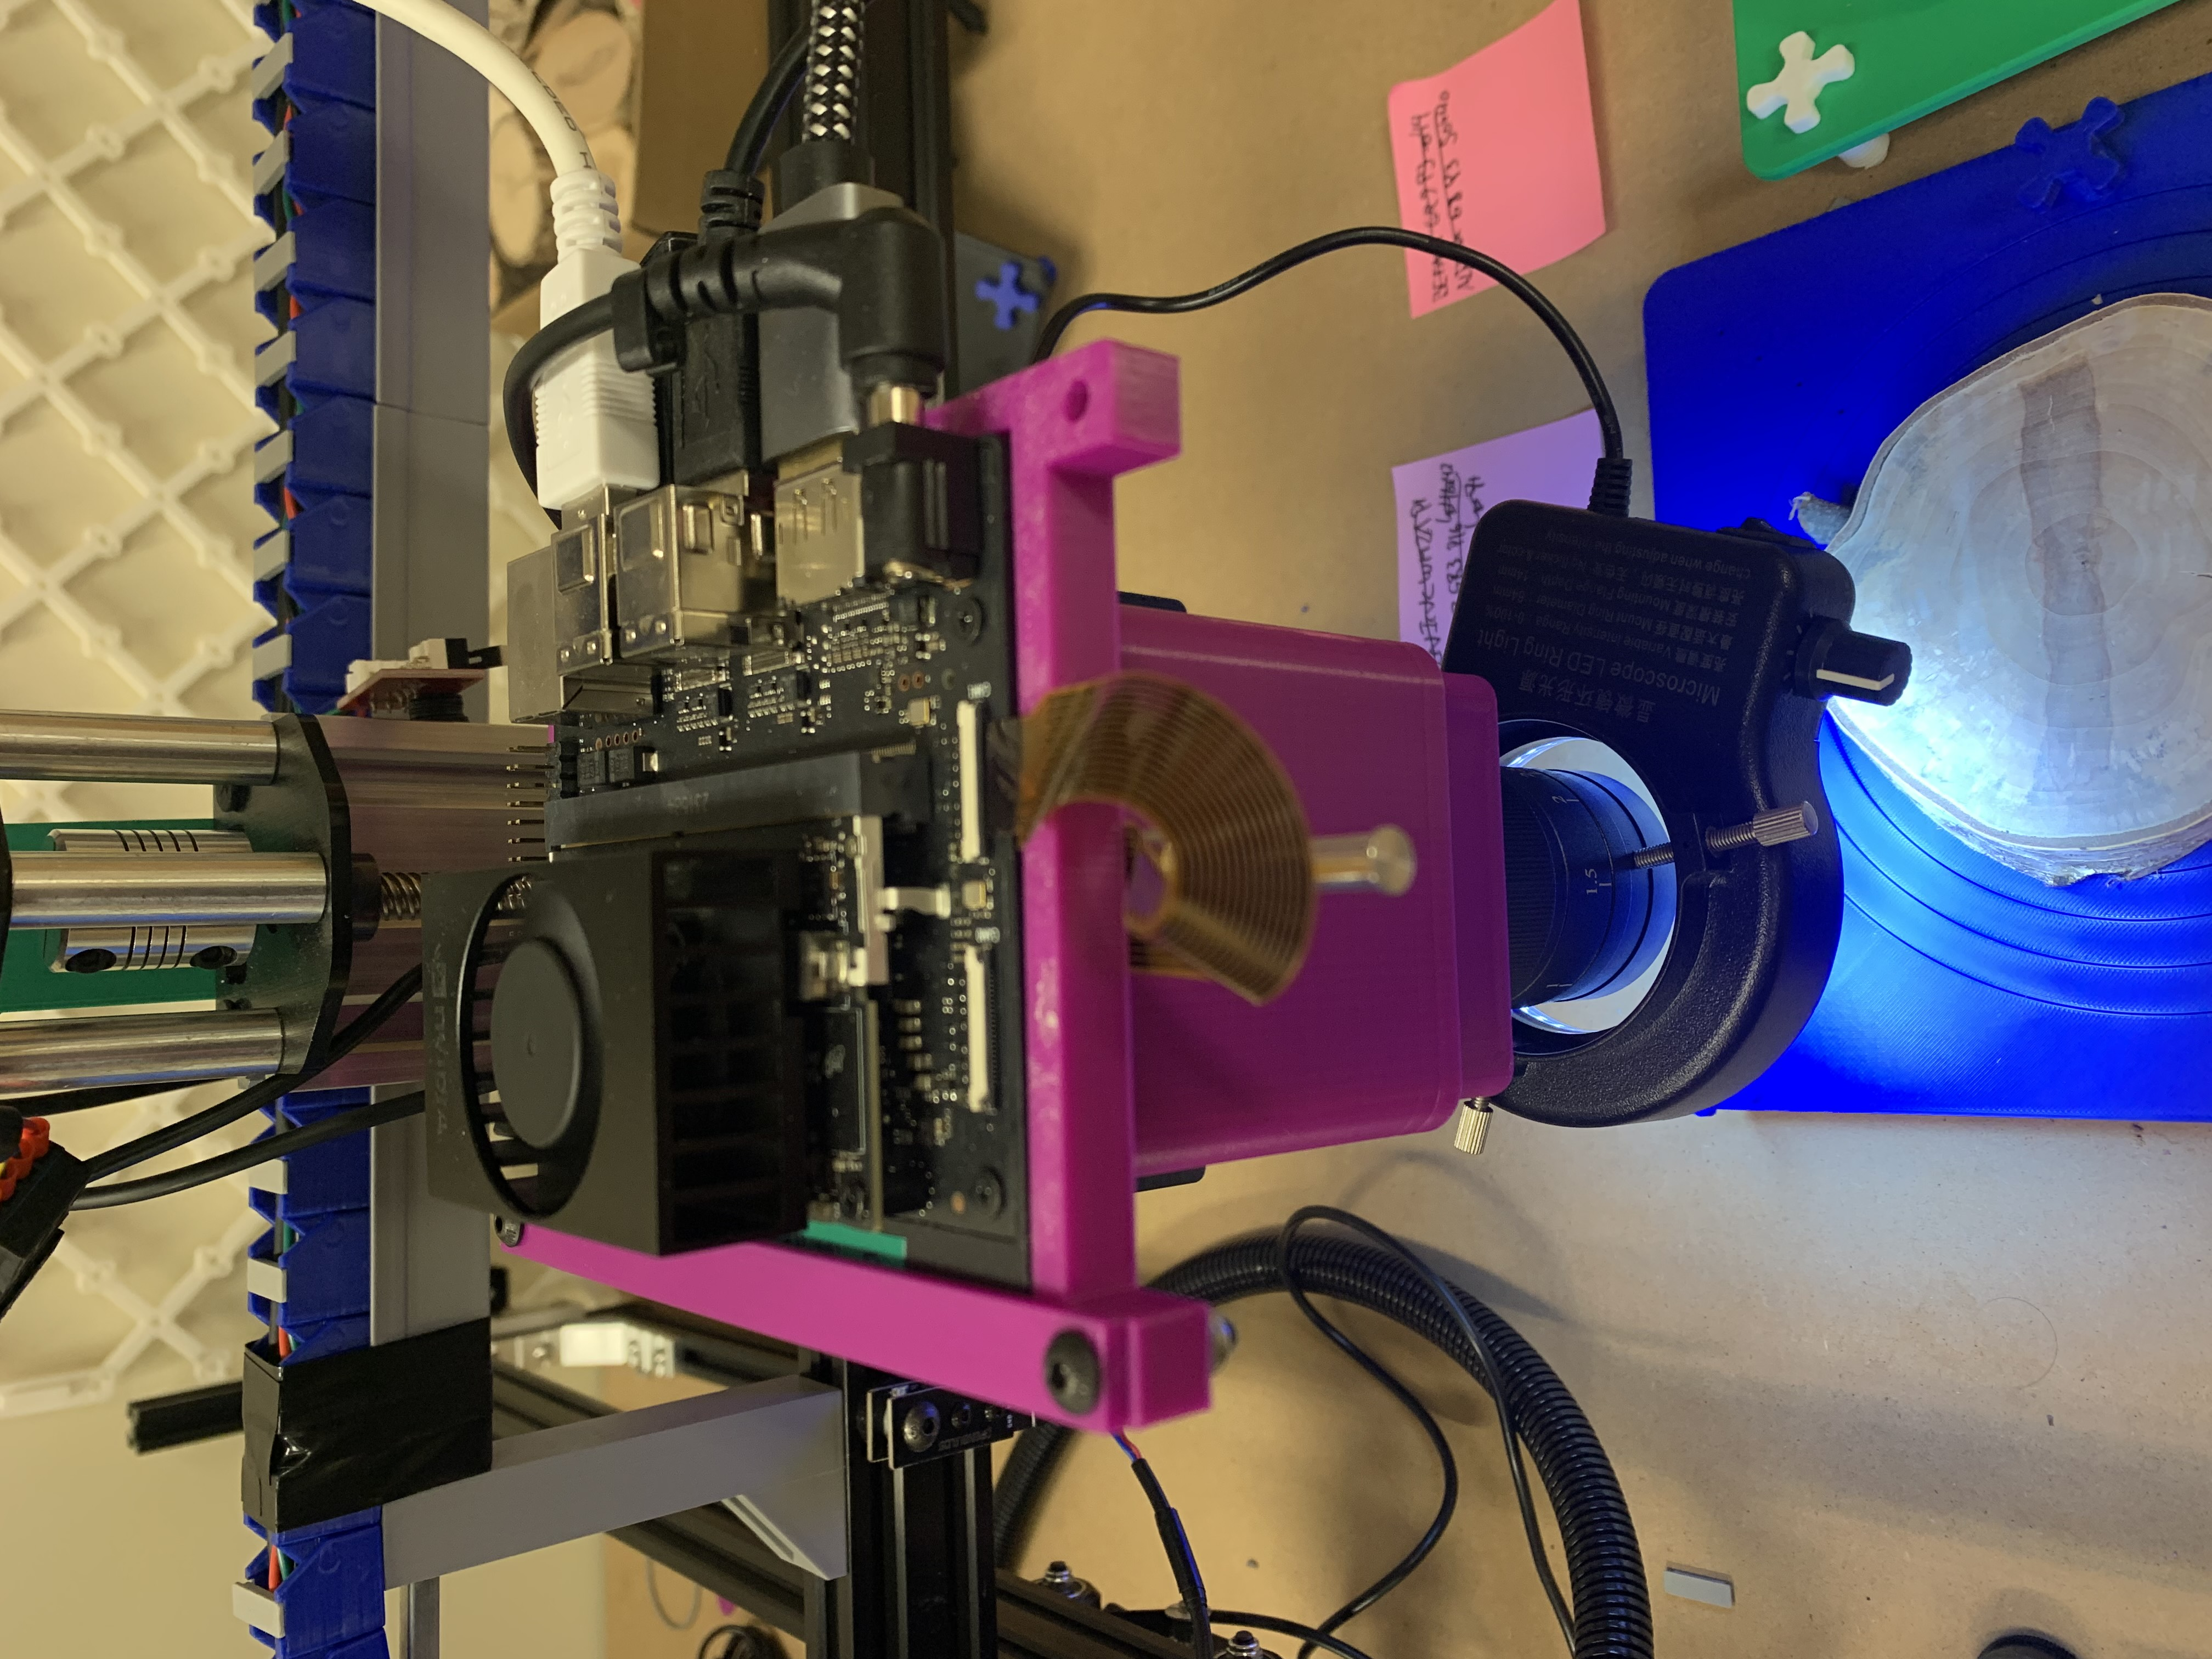
\includegraphics[width=0.5\textwidth,angle=-90]{../docs/content/jetson_on_carriage.jpg}
    \caption{Jetson Orin Nano installed in the carriage with the camera assembly mounted underneath.}
    \label{fig:jetson-carriage}
\end{figure}

\begin{table}[H]
\centering
\begin{tabularx}{\textwidth}{p{2.5cm} X c}
\toprule
\textbf{Component Type} & \textbf{Component Name} & \textbf{Quantity} \\
\midrule

Extra & Jetson Orin Nano & 1 \\
      & Raspberry Pi HQ Camera & 1 \\
      & SEEED Studio Lens & 1 \\
      & CSI cable & 1 \\

\bottomrule
\end{tabularx}
\caption{Components required for camera and computer installation.}
\label{tab:camera-install-components}
\end{table}




\section{Operating TIM}

% Add operating instructions here.

% --------------------------------------------------
\section{References}

\begin{enumerate}[label={[\arabic*]}]

    \item OpenBuilds (2019a). OpenBuilds Acro System Assembly (Mechanical Build) [Video]. YouTube.
    \url{https://www.youtube.com/watch?v=YDLJrxrMEAo}

    \item OpenBuilds (2018). V-Slot\textsuperscript{\textregistered} NEMA 17 Linear Actuator Bundle (Lead Screw) [Video]. YouTube.
    \url{https://www.youtube.com/watch?v=X0Z_gfl-iGY}

    \item OpenBuilds (2019b). OpenBuilds Acro System Electronics and Software (Using BlackBox) [Video]. YouTube.
    \url{https://www.youtube.com/watch?v=GrjqW2MDCvM}

\end{enumerate}

\end{document}
